% Options for packages loaded elsewhere
\PassOptionsToPackage{unicode}{hyperref}
\PassOptionsToPackage{hyphens}{url}
%
\documentclass[
  12pt,
]{article}
\usepackage{amsmath,amssymb}
\usepackage{iftex}
\ifPDFTeX
  \usepackage[T1]{fontenc}
  \usepackage[utf8]{inputenc}
  \usepackage{textcomp} % provide euro and other symbols
\else % if luatex or xetex
  \usepackage{unicode-math} % this also loads fontspec
  \defaultfontfeatures{Scale=MatchLowercase}
  \defaultfontfeatures[\rmfamily]{Ligatures=TeX,Scale=1}
\fi
\usepackage{lmodern}
\ifPDFTeX\else
  % xetex/luatex font selection
    \setmainfont[]{Times New Roman}
\fi
% Use upquote if available, for straight quotes in verbatim environments
\IfFileExists{upquote.sty}{\usepackage{upquote}}{}
\IfFileExists{microtype.sty}{% use microtype if available
  \usepackage[]{microtype}
  \UseMicrotypeSet[protrusion]{basicmath} % disable protrusion for tt fonts
}{}
\makeatletter
\@ifundefined{KOMAClassName}{% if non-KOMA class
  \IfFileExists{parskip.sty}{%
    \usepackage{parskip}
  }{% else
    \setlength{\parindent}{0pt}
    \setlength{\parskip}{6pt plus 2pt minus 1pt}}
}{% if KOMA class
  \KOMAoptions{parskip=half}}
\makeatother
\usepackage{xcolor}
\usepackage[margin=1in]{geometry}
\usepackage{color}
\usepackage{fancyvrb}
\newcommand{\VerbBar}{|}
\newcommand{\VERB}{\Verb[commandchars=\\\{\}]}
\DefineVerbatimEnvironment{Highlighting}{Verbatim}{commandchars=\\\{\}}
% Add ',fontsize=\small' for more characters per line
\usepackage{framed}
\definecolor{shadecolor}{RGB}{248,248,248}
\newenvironment{Shaded}{\begin{snugshade}}{\end{snugshade}}
\newcommand{\AlertTok}[1]{\textcolor[rgb]{0.94,0.16,0.16}{#1}}
\newcommand{\AnnotationTok}[1]{\textcolor[rgb]{0.56,0.35,0.01}{\textbf{\textit{#1}}}}
\newcommand{\AttributeTok}[1]{\textcolor[rgb]{0.13,0.29,0.53}{#1}}
\newcommand{\BaseNTok}[1]{\textcolor[rgb]{0.00,0.00,0.81}{#1}}
\newcommand{\BuiltInTok}[1]{#1}
\newcommand{\CharTok}[1]{\textcolor[rgb]{0.31,0.60,0.02}{#1}}
\newcommand{\CommentTok}[1]{\textcolor[rgb]{0.56,0.35,0.01}{\textit{#1}}}
\newcommand{\CommentVarTok}[1]{\textcolor[rgb]{0.56,0.35,0.01}{\textbf{\textit{#1}}}}
\newcommand{\ConstantTok}[1]{\textcolor[rgb]{0.56,0.35,0.01}{#1}}
\newcommand{\ControlFlowTok}[1]{\textcolor[rgb]{0.13,0.29,0.53}{\textbf{#1}}}
\newcommand{\DataTypeTok}[1]{\textcolor[rgb]{0.13,0.29,0.53}{#1}}
\newcommand{\DecValTok}[1]{\textcolor[rgb]{0.00,0.00,0.81}{#1}}
\newcommand{\DocumentationTok}[1]{\textcolor[rgb]{0.56,0.35,0.01}{\textbf{\textit{#1}}}}
\newcommand{\ErrorTok}[1]{\textcolor[rgb]{0.64,0.00,0.00}{\textbf{#1}}}
\newcommand{\ExtensionTok}[1]{#1}
\newcommand{\FloatTok}[1]{\textcolor[rgb]{0.00,0.00,0.81}{#1}}
\newcommand{\FunctionTok}[1]{\textcolor[rgb]{0.13,0.29,0.53}{\textbf{#1}}}
\newcommand{\ImportTok}[1]{#1}
\newcommand{\InformationTok}[1]{\textcolor[rgb]{0.56,0.35,0.01}{\textbf{\textit{#1}}}}
\newcommand{\KeywordTok}[1]{\textcolor[rgb]{0.13,0.29,0.53}{\textbf{#1}}}
\newcommand{\NormalTok}[1]{#1}
\newcommand{\OperatorTok}[1]{\textcolor[rgb]{0.81,0.36,0.00}{\textbf{#1}}}
\newcommand{\OtherTok}[1]{\textcolor[rgb]{0.56,0.35,0.01}{#1}}
\newcommand{\PreprocessorTok}[1]{\textcolor[rgb]{0.56,0.35,0.01}{\textit{#1}}}
\newcommand{\RegionMarkerTok}[1]{#1}
\newcommand{\SpecialCharTok}[1]{\textcolor[rgb]{0.81,0.36,0.00}{\textbf{#1}}}
\newcommand{\SpecialStringTok}[1]{\textcolor[rgb]{0.31,0.60,0.02}{#1}}
\newcommand{\StringTok}[1]{\textcolor[rgb]{0.31,0.60,0.02}{#1}}
\newcommand{\VariableTok}[1]{\textcolor[rgb]{0.00,0.00,0.00}{#1}}
\newcommand{\VerbatimStringTok}[1]{\textcolor[rgb]{0.31,0.60,0.02}{#1}}
\newcommand{\WarningTok}[1]{\textcolor[rgb]{0.56,0.35,0.01}{\textbf{\textit{#1}}}}
\usepackage{longtable,booktabs,array}
\usepackage{calc} % for calculating minipage widths
% Correct order of tables after \paragraph or \subparagraph
\usepackage{etoolbox}
\makeatletter
\patchcmd\longtable{\par}{\if@noskipsec\mbox{}\fi\par}{}{}
\makeatother
% Allow footnotes in longtable head/foot
\IfFileExists{footnotehyper.sty}{\usepackage{footnotehyper}}{\usepackage{footnote}}
\makesavenoteenv{longtable}
\usepackage{graphicx}
\makeatletter
\def\maxwidth{\ifdim\Gin@nat@width>\linewidth\linewidth\else\Gin@nat@width\fi}
\def\maxheight{\ifdim\Gin@nat@height>\textheight\textheight\else\Gin@nat@height\fi}
\makeatother
% Scale images if necessary, so that they will not overflow the page
% margins by default, and it is still possible to overwrite the defaults
% using explicit options in \includegraphics[width, height, ...]{}
\setkeys{Gin}{width=\maxwidth,height=\maxheight,keepaspectratio}
% Set default figure placement to htbp
\makeatletter
\def\fps@figure{htbp}
\makeatother
\setlength{\emergencystretch}{3em} % prevent overfull lines
\providecommand{\tightlist}{%
  \setlength{\itemsep}{0pt}\setlength{\parskip}{0pt}}
\setcounter{secnumdepth}{5}
% definitions for citeproc citations
\NewDocumentCommand\citeproctext{}{}
\NewDocumentCommand\citeproc{mm}{%
  \begingroup\def\citeproctext{#2}\cite{#1}\endgroup}
\makeatletter
 % allow citations to break across lines
 \let\@cite@ofmt\@firstofone
 % avoid brackets around text for \cite:
 \def\@biblabel#1{}
 \def\@cite#1#2{{#1\if@tempswa , #2\fi}}
\makeatother
\newlength{\cslhangindent}
\setlength{\cslhangindent}{1.5em}
\newlength{\csllabelwidth}
\setlength{\csllabelwidth}{3em}
\newenvironment{CSLReferences}[2] % #1 hanging-indent, #2 entry-spacing
 {\begin{list}{}{%
  \setlength{\itemindent}{0pt}
  \setlength{\leftmargin}{0pt}
  \setlength{\parsep}{0pt}
  % turn on hanging indent if param 1 is 1
  \ifodd #1
   \setlength{\leftmargin}{\cslhangindent}
   \setlength{\itemindent}{-1\cslhangindent}
  \fi
  % set entry spacing
  \setlength{\itemsep}{#2\baselineskip}}}
 {\end{list}}
\usepackage{calc}
\newcommand{\CSLBlock}[1]{\hfill\break\parbox[t]{\linewidth}{\strut\ignorespaces#1\strut}}
\newcommand{\CSLLeftMargin}[1]{\parbox[t]{\csllabelwidth}{\strut#1\strut}}
\newcommand{\CSLRightInline}[1]{\parbox[t]{\linewidth - \csllabelwidth}{\strut#1\strut}}
\newcommand{\CSLIndent}[1]{\hspace{\cslhangindent}#1}
\usepackage{tcolorbox}
\usepackage{amssymb}
\usepackage{yfonts}
\usepackage{bm}
\usepackage{kbordermatrix}
\usepackage{titlesec}


\newtcolorbox{greybox}{
  colback=white,
  colframe=blue,
  coltext=black,
  boxsep=5pt,
  arc=4pt}
  
\newcommand{\sectionbreak}{\clearpage}

 
\newcommand{\ds}[4]{\sum_{{#1}=1}^{#3}\sum_{{#2}=1}^{#4}}
\newcommand{\us}[3]{\mathop{\sum\sum}_{1\leq{#2}<{#1}\leq{#3}}}

\newcommand{\ol}[1]{\overline{#1}}
\newcommand{\ul}[1]{\underline{#1}}

\newcommand{\amin}[1]{\mathop{\text{argmin}}_{#1}}
\newcommand{\amax}[1]{\mathop{\text{argmax}}_{#1}}

\newcommand{\ci}{\perp\!\!\!\perp}

\newcommand{\mc}[1]{\mathcal{#1}}
\newcommand{\mb}[1]{\mathbb{#1}}
\newcommand{\mf}[1]{\mathfrak{#1}}

\newcommand{\eps}{\epsilon}
\newcommand{\lbd}{\lambda}
\newcommand{\alp}{\alpha}
\newcommand{\df}{=:}
\newcommand{\am}[1]{\mathop{\text{argmin}}_{#1}}
\newcommand{\ls}[2]{\mathop{\sum\sum}_{#1}^{#2}}
\newcommand{\ijs}{\mathop{\sum\sum}_{1\leq i<j\leq n}}
\newcommand{\jis}{\mathop{\sum\sum}_{1\leq j<i\leq n}}
\newcommand{\sij}{\sum_{i=1}^n\sum_{j=1}^n}
	
\ifLuaTeX
  \usepackage{selnolig}  % disable illegal ligatures
\fi
\usepackage{bookmark}
\IfFileExists{xurl.sty}{\usepackage{xurl}}{} % add URL line breaks if available
\urlstyle{same}
\hypersetup{
  pdfauthor={Jan de Leeuw - University of California Los Angeles},
  hidelinks,
  pdfcreator={LaTeX via pandoc}}

\title{Smacof at 50: A Manual\\
Part 1: Smacof with B-Splines}
\author{Jan de Leeuw - University of California Los Angeles}
\date{Started February 21 2024, Version of March 31, 2024}

\begin{document}
\maketitle
\begin{abstract}
TBD
\end{abstract}

{
\setcounter{tocdepth}{4}
\tableofcontents
}
\textbf{Note:} This is a working manuscript which will be expanded/updated
frequently. All suggestions for improvement are welcome. All Rmd, tex,
html, pdf, R, and C files are in the public domain. Attribution will be
appreciated, but is not required. The files can be found at
\url{https://github.com/deleeuw/smacofCode}.

\sectionbreak

\section{Introduction}\label{introduction}

In \emph{Multidimensional Scaling (MDS)} the data consists of information
about the similarity or dissimilarity between pairs of objects selected
from a finite set \(\mathcal{O}=\{o_1,\cdots,o_n\}\).

In \emph{metric MDS} we have numerical dissimilarity measures and we want to
map the objects \(o_i\) into \(n\) points \(x_i\) of some metric space in such
a way that the distances between the points approximate the
dissimilarities between the objects. In \emph{smacof}, our framework for MDS
theory, algorithms, and computer programs, the metric space is
\(\mathbb{R}^p\), the space of all \(p\)-tuples of real numbers, and in the
code documented in this manual we assume the distance is the usual
Euclidean distance.

In \emph{non-metric MDS} the information about the dissimilarities is
incomplete. It is usually \emph{ordinal}, i.e.~it tells us in some way or
another that some dissimilarties are larger or smaller than others.
Somewhere between metric and non-metric MDS is MDS with \emph{missing data},
in which some dissimilarities are known numbers while others are
unknown. MDS with missing data is a form of \emph{distance matrix completion}
(Fang and O'Leary (2012)).

\section{Krukal's Stress}\label{krukals-stress}

In the pioneering papers Kruskal (1964a) and Kruskal (1964b) the MDS problem
was formulated for the first time as minimization of an explicit loss
function, which measures the quality of the approximation of the
dissimilarities by the distances.

\subsection{Metric MDS}\label{metric-mds}

The loss function in least squares
metric Euclidean MDS is called \emph{raw stress} or \emph{Kruskal's raw stress}
and is defined as
\begin{equation}
\sigma_R(X):=\frac12\sum w_{ij}(\delta_{ij}-d_{ij}(X))^2.
\label{eq:stressdef}
\end{equation}

The symbol \(:=\) is used for definitions. In definition
\eqref{eq:stressdef} the \(w_{ij}\) are known non-negative \emph{weights}, the
\(\delta_{ij}\) are the known non-negative \emph{dissimilarities} between
objects \(o_i\) and \(o_j\), and the \(d_{ij}(X)\) are the \emph{distances} between
the corresponding points \(x_i\) and \(x_j\). The summation is over all
\(\binom{n}{2}\) pairs \((i,j)\) with \(j>i\), i.e.~over elements below the
diagonal of the matrices \(W\) and \(\Delta\). The subscript \(R\) in \(\sigma_R\)
stands for ``raw''. From now on we use ``metric
MDS'' to mean Least Squares Metric Euclidean MDS.

The \(n\times p\) matrix \(X\), which has the coordinates \(x_i\) of the \(n\)
points as its rows, is called the \emph{configuration}, where \(p\) is the
\emph{dimension} of the Euclidean space in which we make the map. Thus
\begin{equation}
d_{ij}(X)=\sqrt{\sum_{s=1}^p(x_{is}-x_{js})^2}.
\label{eq:ddef}
\end{equation} The metric MDS problem (of dimension \(p\), for given \(W\)
and \(\Delta\)) is the minimization of \eqref{eq:stressdef} over the
\(n\times p\) configurations \(X\).

The weights \(w_{ij}\) can be used to quantify information about the
precision or importance of the corresponding dissimilarities. Some of
the weights may be zero, which can be used to code \emph{missing data}. If
all weights are positive we have \emph{complete data}. If we have complete
data, and all weights are equal to one, we have \emph{unweighted} metric MDS.
The pioneering papers by Shepard, Kruskal, and Guttman only consider the unweighted case. Weights were only introduced in MDS in De Leeuw (1977).

We assume throughout that the weights are \emph{irreducible} (De Leeuw (1977)).
This means there is no partitioning of the index set
\(I_n:=\{1,2,\cdots,n\}\) into subsets for which all between-subset
weights are zero. A reducible metric MDS problems decomposes into a
number of smaller independent metric MDS problems, so the irreducibility
assumption causes no real loss of generality.

The fact that the summation in \eqref{eq:stressdef} is over all \(j<i\)
indicates that the diagonal elements of \(\Delta\) are not used (they are
assumed to be zero) and the elements above the diagonal are not used as
well (they are assumed to be equal to the corresponding elements below
the diagonal). The somewhat mysterious factor \(\frac12\) in definition
\eqref{eq:stressdef} is there because it simplifies some of the formulas
in later sections of this paper.

\subsection{Non-metric MDS}\label{non-metric-mds}

Kruskal was not really interested in metric MDS and the ``raw'' loss
function \eqref{eq:stressdef}. His papers are really about non-metric
MDS, by which we mean least squares non-metric Euclidean MDS. Non-metric
MDS differs from metric MDS because we have incomplete information about
the dissimilarities. As we have seen, that if some dissimilarities are
missing metric MDS can handle this by using zero weights. In some
situations, however, we only know the rank order of the non-missing
dissimilarities. We do not know, or we refuse to use, their actual
numeric values. Or, to put it differently, even if we have numerical
dissimilarities we are looking for a \emph{transformation} of the non-missing
dissimilarities, where the transformation is chosen from a set of
admissible transformations (for instance from all linear or monotone
transformations). If the dissimilarities are non-numerical, for example
rank orders or partitionings, we choose from the set of admissible
\emph{quantifications}.

In non-metric MDS raw stress becomes
\begin{equation}
\sigma_R(X,\Delta):=\frac12\sum w_{ij}(\delta_{ij}-d_{ij}(X))^2,
\label{eq:rawstressdef}
\end{equation}
where \(\Delta\) varies over the quantified or transformed
dissimilarities. In MDS parlance they are also called \emph{pseudo-distances}
or \emph{disparities}. Loss function \eqref{eq:rawstressdef} must be minimized
over both configurations and disparities, with the condition that the
disparities \(\Delta\) are an admissible transformation or quantification
of the data. In Kruskal's non-metric MDS this means
requiring monotonicity. In this paper we will consider various other
choices for the set of admissible transformations. We will use the
symbol \(\mathfrak{D}\) for the set of admissible transformations

The most familiar examples of \(\mathfrak{D}\) (linear,
polynomial, splines, monotone) define convex cones with apex at the origin. This
means that if \(\Delta\in\mathfrak{D}\) then so is \(\lambda\Delta\) for all
\(\lambda\geq 0\). But consequently minimizing \eqref{eq:rawstressdef} over
all \(\Delta\in\mathfrak{D}\) and over all configurations has the trivial
solution \(\Delta=0\) and \(X=0\), corresponding with the global minimum
\(\sigma(X,\Delta)=0\). We need additional constraints to rule out this
trivial solution, and in non-metric MDS this is done by choosing a
\emph{normalization} that keeps the solution away from zero.

Kruskal's original solution is to define \emph{normalized stress} as
\begin{equation}
\sigma(X,\Delta):=\frac{\sum w_{ij}(\delta_{ij}-d_{ij}(X))^2}{\sum w_{ij}d_{ij}^2(X)}.
\label{eq:nstressdef}
\end{equation}
To be precise, in Kruskal's formulation there are no weights,
and he actually takes the square root of \eqref{eq:nstressdef} to define
\emph{Kruskal's stress}. The non-metric Euclidean MDS problem now is to minimize
loss function \eqref{eq:nstressdef} over all \(n\times p\) configurations
\(X\) and all admissible disparities \(\Delta\).

\subsection{Normalization}\label{normalization}

Equation \eqref{eq:nstressdef} is only one way to normalize raw stress. Some obvious alternatives are discussed in detail in
Kruskal and Carroll (1969) and De Leeuw (1975). In the terminology of
De Leeuw (1975) there are \emph{explicit} and \emph{implicit} normalizations.

In implicit normalization we minimize either
\begin{equation}
\sigma(X,\hat D):=\frac{\sum  w_{ij}(\hat d_{ij} -d_{ij}(X))^2}{\sum   w_{ij}^{\ }\hat d_{ij}^2}
\label{eq:implicit1}
\end{equation}
or
\begin{equation}
\sigma(X,\hat D):=\frac{\sum   w_{ij}(\hat d_{ij}-d_{ij}(X))^2}{\sum   w_{ij}^{\ }d_{ij}^2(X) }
\label{eq:implicit2}
\end{equation}
over \(X\) and \(\Delta\in\mathfrak{D}\).

As we have seen, Kruskal (1964a) chooses definition \eqref{eq:implicit2} and
calls the explicitly normalized loss function \emph{normalized stress}. Note that we overload the symbol \(\sigma\) to denote any one of the least squares loss
functions. It will always be clear from the text which \(\sigma\) we are
talking about.

In explicit normalization we minimize the raw stress \(\sigma_R(X,\hat D)\)
from \eqref{eq:rawstressdef}, but we add the explicit constraint
\begin{equation}
\sum   w_{ij}^{\ }d_{ij}^2(X)=1,
\label{eq:explicit1}
\end{equation}
or the constraint
\begin{equation}
\sum   w_{ij}^{\ }\hat d_{ij}^2=1.
\label{eq:explicit2}
\end{equation}
Kruskal and Carroll (1969) and De Leeuw (2019) show that these
four normalizations all lead to essentially the same solution for \(X\)
and \(\hat D\), up to scale factors dictated by the choice of the particular
normalization. It is also possible to normalize both \(X\) and \(\hat D\),
either explicitly or implicitly, and again this will give the same
solutions, suitably normalized. These invariance results assume the
admissible transformations form a closed cone with apex at the origin,
i.e.~if \(\hat D\) is admissible and \(\lambda\geq 0\) then \(\lambda\hat D\)
is admissible as well. The matrices of Euclidean distances \(D(X)\) form a
similar closed cone as well. The non-metric MDS problem is to find an element
of the \(\hat D\) cone \(\mathcal{D}\) and an element of the \(D(X)\) cone where the angle between the two is a small as possible.

In the R version of smacof (De Leeuw and Mair (2009),
Mair, Groenen, and De Leeuw (2022)) we use explicit normalization
\eqref{eq:explicit2}. This is supported by the result, also due to
De Leeuw (1975), that projection on the intersection of the cone of
disparities and the sphere defined by \eqref{eq:explicit2} is equivalent
to first projecting on the cone and then normalizing the projection (see
also Bauschke, Bui, and Wang (2018)).

In the version of non-metric MDS discussed in this manualwe need more flexibility. For algorithmic reasons that may become clear later on, we will go with the original \eqref{eq:nstressdef}, i.e.~with the implicitly normalized
Kruskal's stress. For the final results the choice between normalizations should not make a difference, but the iterative computations will be different for the
diufferent choices.

\subsection{Some thoughts on ALS}\label{some-thoughts-on-als}

I will take this opportunity to clear up some misunderstandings and
confusions that have haunted the early development of non-metric MDS.

\subsubsection{The Single-Phase approach}\label{the-single-phase-approach}

In Kruskal (1964a) defines
\begin{equation}
\sigma(X):=\min_{\hat D\in\mathfrak{D}}\ \sigma(\hat D,X)=\sigma(X,\hat D(X)),
\label{eq:project}
\end{equation}
where \(\sigma(\hat D,X)\) is defined by
\eqref{eq:implicit2}. The minimum in \eqref{eq:project} is over admissible
transformations. In definition \eqref{eq:project}
\begin{equation}
\hat D(X):=\mathop{\text{argmin}}_{\hat D\in\mathfrak{D}}\sigma(X, \hat D).
\label{eq:optscal}
\end{equation}
Normalized stress defined by \eqref{eq:project} is now a
function of \(X\) only. Under some conditions, which are true in Kruskal's
definition of non-metric MDS, there is a simple relation between the
partials of \eqref{eq:implicit2} and those of \eqref{eq:project}.
\begin{equation}
\mathcal{D}\sigma(X)=\mathcal{D}_1\sigma(X,\hat D(X)),
\label{eq:partials}
\end{equation}
where \(\mathcal{D}\sigma(X)\) are the derivatives of
\(\sigma\) from \eqref{eq:project} and \(\mathcal{D}_1\sigma(X,\hat D(X))\)
are the partial derivatives of \(\sigma\) from \eqref{eq:implicit2} with
respect to \(X\). Thus the partials of \(\sigma\) from \eqref{eq:project} can
be computed by evaluating the partials of \(\sigma\) from
\eqref{eq:implicit2} with respect to \(X\) at \((X,\hat D(X))\). This has
created much confusion in the past. The non-metric MDS problem in Kruskal's original formulation is now to
minimize \(\sigma\) from \eqref{eq:project}, which is a function of \(X\)
alone.

Guttman (1968) calls this the \emph{single-phase approach}. A variation of
Kruskal's single-phase approach defines
\begin{equation}
\sigma(X)=\sum w_{ij}(d_{ij}^\#(X)-d_{ij}(X))^2,
\label{eq:rankimage}
\end{equation}
where the \(d_{ij}^\#(X)\) are \emph{Guttman's rank images}, i.e.~the
permutation of the \(d_{ij}(X)\) that makes them monotone with the
\(\delta_{ij}\) (Guttman (1968)). Or, alternatively, define
\begin{equation}
\sigma(X):=\sum   w_{ij}(d_{ij}^\%(X)-d_{ij}(X))^2,
\label{eq:shepard}
\end{equation}
where the \(\hat d_{ij}^\%(X)\) are \emph{Shepard's rank images}, i.e.~the
permutation of the \(\delta_{ij}\) that makes them monotone with the
\(d_{ij}(X)\) (Shepard (1962a), Shepard (1962b), De Leeuw (2017b)).

Minimizing the Shepard or Guttman single-phase loss functions is
computationally more complicated than Kruskal's \emph{monotone regression}
approach, mostly because the rank-image transformations are not
differentiable, and there is no analog of \eqref{eq:partials} and of the
equivalence of the different implicit and explicit normalizations.

\subsubsection{The Two-Phase Approach}\label{the-two-phase-approach}

The \emph{two-phase approach} or \emph{alternating least squares (ALS)} approach
alternates minimization of \(\sigma(\hat D,X)\) over \(X\) for our current
best estimate of \(\hat D\) with minimization of \(\sigma(\hat D,X)\) over
\(\Delta\in\mathfrak{D}\) for our current best value of \(X\). Thus an
update from iteration \(k\) to iteration \(k+1\) looks like \begin{align}
\hat D^{(k)}&=\mathop{\text{argmin}}_{\hat D\in\mathfrak{D}}\sigma(\hat D,X^{(k)}),\label{eq:step1}\\
X^{(k+1)}&=\mathop{\text{argmin}}_X\sigma(\hat D^{(k)},X).\label{eq:step2}
\end{align} This ALS approach to MDS was in the air since the early
(unsuccessful) attempts around 1968 of Young and De Leeuw to combine
Torgerson's classic metric MDS method with Kruskal's monotone regression
transformation. All previous implementations of non-metric smacof use
the two-phase approach, and we will do the same in this paper.

As formulated, however, there are some problems with the ALS algorithm.
Step \eqref{eq:step1} is easy to carry out, using monotone regression.
Step \eqref{eq:step2} means solving a metric scaling problem, which is an
iterative proces that requires an infinite number of iterations. Thus,
in the usual implementations, step \eqref{eq:step1} is combined with one
of more iterations of a convergent iterative procedure for metric MDS,
such as smacof. If we take only one of these \emph{inner iterations} the
algorithm becomes indistinguishable from Kruskal's single-phase method.
This has also created much confusion in the past.

In the usual implementations of the ALS approach we solve the first
subproblem \eqref{eq:step1} exactly, while we take only a single step
towards the solution for given \(\hat D\) in the second phase
\eqref{eq:step2}. If we have an infinite iterative procedure to compute
the optimal \(\hat D\in\mathfrak{D}\) for given \(X\), then a more balanced
approach would be to take several inner iterations in the first phase
and several inner iterations in the second phase. How many of each,
nobody knows. In our current implementation of smacof we take several
inner iteration steps in the first phase and a single inner iteration
step in the second phase.

\section{Smacof Notation and Terminology}\label{smacof-notation-and-terminology}

We discuss some standard MDS notation, first introduced in
De Leeuw (1977). This notation is useful for the second phase of the ALS
algorithm, in which solve the metric MDS problem of we minimizing
unnormalized \(\sigma(X,\hat D)\) over \(X\) for fixed \(\hat D\). We will
discuss the first ALS phase later in the paper.

Start with the unit vectors \(e_i\) of length \(n\). They have a non-zero
element equal to one in position \(i\), all other elements are zero. Think
of the \(e_i\) as the columns of the identity matrix.

Using the \(e_i\) we define for all \(i\not= j\) the matrices
\begin{equation}
A_{ij}:=(e_i-e_j)(e_i-e_j)'.
\end{equation} The \(A_{ij}\) are of order \(n\), symmetric,
doubly-centered, and of rank one. They have four non-zero elements.
Elements \((i,i)\) and \((j,j)\) are equal to \(+1\), elements \((i,j)\) and
\((j,i)\) are \(-1\).

The importance of \(A_{ij}\) in MDS comes from the equation
\begin{equation}
d_{ij}^2(X)=\text{tr}\ X'A_{ij}X.
\label{eq:dfroma}
\end{equation} In addition we use the fact that the \(A_{ij}\) form a
basis for the \(binom{n}{2}\)-dimensional linear space of all
doubly-centered symmetric matrices.

Expanding the square in the definition of stress gives \begin{equation}
\sigma(X)=\frac12\{\sum   w_k\delta_k^2-2\ \sum   w_k\delta_kd_k(X)+\sum   w_kd_k^2(X)\}.
\label{eq:expand}
\end{equation} It is convenient to have notation for the three separate
components of stress from equation \eqref{eq:expand}. Define
\begin{align}
\eta_{\hat D}^2&=\sum   w_{ij}\hat d_{ij}^2,\label{eq:condef}\\
\rho(X)&=\sum   w_{ij}\hat d_{ij}d_{ij}(X),\label{eq:rhodef}\\
\eta^2(X)&=\sum   w_{ij}d_{ij}(X)^2.\label{eq:etadef}
\end{align} which lead to \begin{equation}
\sigma(X)=\frac12\left\{\eta_{\hat D}^2-2\rho(X)+\eta^2(X)\right\}.
\label{eq:stressshort}
\end{equation} We also need \begin{equation}
\lambda(X)=\frac{\rho(X)}{\eta(X)}.
\label{eq:lambdadef}
\end{equation}

Using the \(A_{ij}\) makes it possible to give matrix expressions for
\(\rho\) and \(\eta^2\). First \begin{equation}
\eta^2(X)=\text{tr}\ X'VX,
\label{eq:etamat}
\end{equation} with \begin{equation}
V:=\sum   w_{ij}A_{ij}.
\label{eq:vdef}
\end{equation} In the same way \begin{equation}
\rho(X)=\text{tr}\ X'B(X)X,
\label{eq:rhomat}
\end{equation} with \begin{equation}
B(X):=\sum   w_{ij}r_{ij}(X)A_{ij},
\label{eq:bdef}
\end{equation} with \begin{equation}
r_{ij}(X):=\begin{cases}\frac{\delta_{ij}}{d_{ij}(X)}&\text{ if }d_{ij}(X)>0,\\
0&\text{ if }d_{ij}(X)=0.
\end{cases}
\end{equation} Note that \(B\) is a function from the set of \(n\times p\)
configurations into the set of symmetric doubly-dentered matrices of
order \(n\). All matrices of the form \(\sum x_{ij}A_{ij}\), where summation
is over all pairs \((i,j)\) with \(j<i\), are symmetric and doubly-centered.
They have \(-x_{ij}\) as off-diagonal elements while the diagonal elements
\((i,i)\) are \(\sum_{j=1}^nx_{ij}\).

Because \(B(X)\) and \(V\) are non-negative linear combinations of the
\(A_{ij}\) they are both positive semi-definite. Because \(W\) is assumed to
be irreducible the matrix \(V\) has rank \(n-1\), with only vectors
proportional to the vector \(e\) with all elements equal to one in its
null-space (De Leeuw (1977)).

Summarizing the results so far we have \begin{equation}
\sigma(X)=\frac12\{\eta_{\hat D}^2-\text{tr}\ X'B(X)X+\text{tr}\ X'VX\}.
\label{eq:sigmat}
\end{equation}

Next we define the \emph{Guttman transform} of a configuration \(X\), for given
\(W\) and \(\Delta\), as \begin{equation}
G(X)=V^+B(X)X,
\label{eq:gudef}
\end{equation} with \(V^+\) the Moore-Penrose inverse of \(V\). In our
computations we use \[
V^+=(V+\frac{1}{n}ee')^{-1}-\frac{1}{n}ee'
\] Also note that in the unweighted case with complete data \(V=nJ\),
where \(J\) is the centering matrix \(I-\frac{1}{n}ee'\), and thus
\(V^+=\frac{1}{n}J\). The Guttman transform is then simply
\(G(X)=n^{-1}B(X)X\).

\section{Intermezzo: Explicit Normalization}\label{intermezzo-explicit-normalization}

\[
\sigma(X,\hat D)=\frac12\frac{\sum w_{ij}(\hat d_{ij}-d_{ij}(X))^2}{\sum w_{ij}d_{ij}^2(X)}
\]
Majorize

\[
\sigma(X,\hat D)\leq\frac12\frac{\eta^2(\hat D)-2\text{tr}\ X'V\overline{Y}+\text{tr}\ X'VX}{\text{tr}\ X'VX}=\frac{\omega(X,Y)}{\eta^2(X)}
\]
Stationary equations
\[
\eta^2(X)(VX-VG(Y))-\omega(X,Y)VX=V\{(\eta^2(X)-\omega(X,Y))X-\eta^2(X)\overline Y\}
\]
So at a minimum \(X\) is proportional to \(\overline{Y}\) or \(X=\alpha\overline{Y}\) for some \(\alpha\). For \ldots{} to be zero we must have
\[
\alpha(\alpha^2\eta^2(\overline Y)-(\eta^2(\hat D)-2\alpha\eta^2(\overline Y)+\alpha^2\eta^2(\overline Y))=\alpha^2\eta^2(\overline Y)
\]
which works out to be
\[
\alpha=\frac{\eta^2(\hat D)}{\eta^2(\overline Y)}
\]
\[
\hat X=\frac{\eta^2(\hat D)}{\eta^2(\overline Y)}\ \overline{Y}
\]
The minimum is equal to

\[
\frac{-\frac{(\eta^2(\overline Y))^2}{\eta^2(\hat D)}+\eta^2(\overline Y)}{\eta^2(\overline Y)}=1-\frac{\eta^2(\overline Y)}{\eta^2(\hat D)}
\]
Use homogeneity of the Guttman transform.

More generally suppose we update with
\[
X=\overline Y+\alpha(Y-\overline Y)
\]
Write
\[
\omega(X,Y)=\eta^2(\hat D)+\text{tr}\ (X-\overline Y)'V(X-\overline Y)-\eta^2(\overline Y)
\]
Thus if \(X(\alpha)=\overline Y+\alpha(Y-\overline Y)\) we have
\[
\omega(\alpha)=\eta^2(\hat D)+\alpha^2\text{tr}\ (Y-\overline Y)'V(Y-\overline Y)-\eta^2(\overline Y)
\]
and
\[
\eta^2(\alpha)=\eta^2(\overline Y)+2\alpha\text{tr}\ (Y-\overline Y)'V\overline Y+\alpha^2\text{tr}\ (Y-\overline Y)'V(Y-\overline Y)
\]
\[
\omega(Y,Y)=\eta^2(\hat D)+\text{tr}\ (Y-\overline Y)'V(Y-\overline Y)-\eta^2(\overline Y)
\]
\[
\frac{\omega(\alpha)}{\eta^2(\alpha)}\leq\sigma(Y)
\]

\section{Properties of Smacof Loss}\label{properties-of-smacof-loss}

\subsection{Derivatives}\label{derivatives}

The Euclidean distance function \(d_{ij}\) from \ldots{} is not differentiable
at configurations \(X\) with \(x_i=x_j\). If \(d_{ij}(X)>0\) then \[
\mathcal{D}\sigma(X)=\frac{1}{d_{ij}(X)}A_{ij}X
\] If \(d_{ij}(X)=0\) then \[
D_+d_{ij}(X,Y)=\lim_{\epsilon\downarrow 0}\frac{d_{ij}(X+\epsilon Y)-d_{ij}(X)}{\epsilon}=d_{ij}(Y)
\] which is non-linear in \(Y\), showing non-differentiability.

\[
D_+\sigma(X,Y)=\text{tr}\ Y'(V-B(X))X+\sum\{w_{ij}\delta_{ij}d_{ij}(Y)\mid d_{ij}(X)=0\}
\] This form of the directional derivative is used by De Leeuw (1984) to
show that two independent necessary conditions for a local minimum are
\((V-B(X))X=0\) and \(d_{ij}(X)>0\) for all \((i,j)\) with
\(w_{ij}\delta_{ij}>0\). \#\#\# Gradient

\[
\mathcal{D}\sigma(X)=(V-B(X))X
\] At a stationary point \(B(X)X=VX\) or \(V^+B(X)X=X\). Thus a necessary
condition for a local minimum is that \(V^+B(X)\) has at least \(p\)
eigenvalues equal to one. De Leeuw (2014) has shown that if
\(V^+B(X)\lesssim I\) then actually \(X\) is a global minimizer of stress.

\subsubsection{Hessian}\label{hessian}

The results on the Hessian of stress are largely unpublished. So we
summarize them here in this manual, so they'll be even more unpublished.

\[
H_{st}(X):=\sum w_{ij}\frac{\delta_{ij}}{d_{ij}(X)}\left\{\frac{A_{ij}x_sx_t'A_{ij}}{d_{ij}^2(X)}\right\}
\]

\[
H_{st}(X)=\sum   w_{ij}\frac{\delta_{ij}}{d_{ij}^3(X)}(x_{is}-x_{js})(x_{it}-x_{jt})A_{ij}
\] \[
\mathcal{D}_{st}\sigma(X)=\begin{cases}H_{st}(X)&\text{ if }s\not= t,\\
V-B(X)+H_{st}&\text{ if }s= t.
\end{cases}
\] If \(I_p\) is the identity matrix of order \(p\), and \(\otimes\) is the
Kronecker product, then \[
\mathcal{D}^2\sigma(X)=I_p\otimes(V - B(X))+ H(X)
\] \[
\sum_{s=1}^p\sum_{t=1}^p y_s'H_{st}y_t=\sum w_{ij}\frac{\delta_{ij}}{d_{ij}(X)}\left\{\frac{(\text{tr} \ Y'A_{ij}X)^2}{d_{ij}^2(X)}\right\}\leq\sum w_{ij}\frac{\delta_{ij}}{d_{ij}(X)}\text{tr}\ Y'A_{ij}Y=\text{tr}\ Y'B(X)Y.
\] Thus \[
0\lesssim H\lesssim I_p\otimes B(X),
\] and \[
I_p\otimes (V-B(X))\lesssim\mathcal{D}^2\sigma(X)\lesssim I_p\otimes V
\] At a local minimum of \(\sigma\) \[
0\lesssim\mathcal{D}^2\sigma(X)\lesssim I_p\otimes V
\] In comparing the lower bounds on \(\mathcal{D}^2\sigma(X)\) in \ldots{} and
\ldots{} De Leeuw (2014) shows that \(V-B(X)\gtrsim 0\) is sufficient for a
\emph{global} minimum of stress (but far from necessary).

Also \[
\sum_{t=1}^p H_{st}y_t=\sum w_{ij}\frac{\delta_{ij}}{d_{ij}(X)}\left\{\frac{\text{tr}\ Y'A_{ij}X }{d_{ij}^2(X)}\right\}A_{ij}x_s
\] If \(Y=X\) then \(H(X)y=(I_p\otimes B(X))x\) and thus
\[\mathcal{D}^2\sigma(X)x=(I_p\otimes V)x.\] In the unweighted case this
means that \(X\) is an eigenvector of \(\mathcal{D}^2\sigma(X)\) with
eigenvalue \(n\). Inequalities \ldots{} show that this is actually the largest
eigenvalue. Or \((I_p\otimes V)^+\mathcal{D}^2\sigma(X)\lesssim I\).

If \(Y=XT\) with \(T\) anti-symmetric then \(\text{tr}\ Y'A_{ij}X=0\) then
thus \(H(X)y=0\). Thus \[
\sum_{t=1}^p\mathcal{D}_{st}\sigma(X)y_t=(V-B(X))y_t
\] which is zero if \(\mathcal{D}\sigma(X)\) is zero. Thus at a stationary
point of stress \(\mathcal{D}^\sigma(X)\) has \(\frac12p(p-1)\) zero
eigenvalues.

There are several ways to think of the Hessian. The simplest one
(perhaps) is as an \(np\times np\) symmetric matrix (corresponding to

column-major R vector of length \(\frac12 np(np+1)\)). This is what we
would use for a straightforward version of Newton-Raphson.

It is more elegant, however, to think of \(H\) as a symmetric super-matrix
of order \(p\), with as elements \(n\times n\) matrices. And, for some
purposes, such as the pseudo-confidence ellipsoids in De Leeuw (2017a), as
a super-matrix of order \(n\) with as elements \(p\times p\) matrices. Both
the super-matrix interpretations lead to four-dimensional arrays, the
first a \(p\times p\times n\times n\) array, the second an
\(n\times n\times p\times p\) array. The different interpretations lead to
different ways to store the Hessian in memory, and to different ways to
retrieve its elements. Of course we can write routines to transform from
one interpretation to another.

\subsection{Lagrangian}\label{lagrangian}

In our implementation of the smacof algorithm we minimize stress over
configurations with \(\eta(X)=1\), or, equivalently,
\(\sum w_{ij}d_{ij}^2(X)=1\). This means we do not look for \(X\) with
\(\mathcal{D}\sigma(X)=(V-B(X))X=0\), but we look for solutions of \[
(V-B(X))X-\lambda VX=0,\\
\text{tr}\ X'VX= 1.
\] At the solution \[
\lambda=1-\rho(X)
\] and \[
X = \frac{\Gamma(X)}{\eta(\Gamma(X))}
\] Also it is necessary for a local minimum that \[
\Gamma(X)=\rho(X)X
\] Because the Guttman transform is homogeneous of degree zero this
implies \[
\Gamma(\Gamma(X)=\Gamma(X),
\] so although \(X\) is not a fixed point of the Guttman transform,
\(\Gamma(X)\) is.

The second order necessary condition is that \[
H(X)\gtrsim I_p\otimes (\rho(X)V - B(X))
\] is positive

\subsubsection{Kuhn-Tucker Points}\label{kuhn-tucker-points}

bozo

\section{Smacof Algorithm}\label{smacof-algorithm}

\subsection{First Phase: Update Configuration}\label{first-phase-update-configuration}

\subsubsection{Introduction to Majorization}\label{introduction-to-majorization}

Majorization, more recently better known as MM (Lange (2016)), is a general
approach for the construction of minimization algorithms. There is also
minorization, which leads to maximization algorithms, which explains the
MM acronym: minorization for maximization and majorization for
minimization.

Before the MM principle was formulated as a general approach to
algorithm construction there were some important predecessors. Major
classes of MM algorithms avant la lettre were the \emph{EM Algorithm} for
maximum likelihood estimation of Dempster, Laird, and Rubin (1977), the \emph{Smacof
Algorithm} for MDS of De Leeuw (1977), the \emph{Generalized Weiszfeldt Method}
of Vosz and Eckhardt (1980), and the \emph{Quadratic Approximation Method} of
Böhning and Lindsay (1988). The first formulation of the general majorization
principle seems to be De Leeuw (1994).

Let's start with a brief introduction to majorization. Minimize a real
valued function \(\sigma\) over \(x\in\mathbb{S}\), where \(\mathbb{S}\) is
some subset of \(\mathbb{R}^n\). There are obvious extensions of
majorization to functions defined on more general spaces, with values in
any partially ordered set, but we do not need that level of generality
in this manual. Also majorization applied to \(\sigma\) is minorization
applied to \(-\sigma\), so concentrating on majorization-minimization and
ignoring minorization-maximization causes no loss of generality

Suppose there is a real-valued function \(\eta\) on
\(\mathbb{S}\otimes\mathbb{S}\) such that

\begin{align}
\sigma(x)&\leq\eta(x,y)\qquad\forall x,y\in\mathbb{S},\label{eq:maj1}\\
\sigma(x)&=\eta(x,x)\qquad\forall x\in\mathbb{S}.\label{eq:maj2}
\end{align}

The function \(\eta\) is called a \emph{majorization scheme} for \(\sigma\) on
\(S\). A majorization scheme is \emph{strict} if \(\sigma(x)<\eta(x,y)\) for all
\(x,y\in S\) withj \(x\not=y\).

Define \begin{equation}
x^{(k+1)}\in\mathop{\text{argmin}}_{x\in\mathbb{S}}\eta(x,x^{(k)}),
\label{eq:majalg}
\end{equation} assuming that \(\eta(\bullet,y)\) attains its (not
necessarily unique) minimum over \(x\in\mathbb{S}\) for each \(y\). If
\(x^{(k)}\in\mathop{\text{argmin}}_{x\in\mathbb{S}}\eta(x,x^{(k)})\) we
stop.

If we do not stop, then by update rule \eqref{eq:majalg} \begin{equation}
\sigma(x^{(k+1)})\leq\eta(x^{(k+1)},x^{(k)}),
\end{equation} by majorization property \eqref{eq:maj1} \begin{equation}
\eta(x^{(k+1)},x^{(k)})\leq\eta(x^{(k)},x^{(k)}).
\end{equation} and by majorization property \eqref{eq:maj1}
\begin{equation}
\eta(x^{(k)},x^{(k)})=\sigma(x^{(k)}).
\end{equation}

If the minimum in \eqref{eq:majalg} is attained for a unique \(x\) then
\(\eta(x^{(k+1)},x^{(k)})<\eta(x^{(k)},x^{(k)})\). If the majorization
scheme is strict then \(\sigma(x^{(k+1)})<\eta(x^{(k+1)},x^{(k)})\). Under
either of these two additional conditions
\(\sigma(x^{(k+1)})<\sigma(x^{(k)})\), which means that the majorization
algorithm is a monotone descent algorithm, and if \(\sigma\) is bounded
below on \(\mathbb{S}\) then the sequence \(\sigma(x^{(k)})\) converges.

Note that we only use the order relation to prove convergence of the
sequence of function values. To prove convergence of the \(x^{(k)}\) we
need stronger compactness and continuity assumptions to apply the
general theory of Zangwill (1969). For such a proof the argmin in update
formula \eqref{eq:majalg} can be generalized to
\(x^{(k+1)}=\phi(x^{(k)})\), where \(\phi\) maps \(\mathbb{S}\) into
\(\mathbb{S}\) such that \(\eta(\phi(x),x)\leq\sigma(x)\) for all \(x\).

We give a small illustration in which we minimize \(\sigma\) with
\(\sigma(x)=\sqrt{x}-\log{x}\) over \(x>0\). Obviously we do not need
majorization here, because solving \(\mathcal{D}\sigma(x)=0\) immediately
gives \(x=4\) as the solution we are looking for.

To arrive at this solution using majorization we start with
\begin{equation}
\sqrt{x}\leq\sqrt{y}+\frac12\frac{x-y}{\sqrt{y}},
\label{eq:sqrtmaj}
\end{equation} which is true because a differentiable concave function
such as the square root is majorized by its tangent everywhere.
Inequality \eqref{eq:sqrtmaj} implies \begin{equation}
\sigma(x)\leq\eta(x,y):=\sqrt{y}+\frac12\frac{x-y}{\sqrt{y}}-\log{x}.
\label{eq:examplemaj}
\end{equation} Note that \(\eta(\bullet,y)\) is convex in its first
argument for each \(y\). We have \(\mathcal{D}_1\eta(x,y)=0\) if and only if
\(x=2\sqrt{y}\) and thus the majorization algorithm is \begin{equation}
x^{(k+1)}=2\sqrt{x^{(k)}}
\label{eq:examplealg}
\end{equation} The sequence \(x^{(k)}\) converges monotonically to the
fixed point \(x=2\sqrt{x}\), i.e.~to \(x=4\). If \(x^{(0)}<4\) the sequence is
increasing, if \(x^{(0)}<4\) it is decreasing. Also, by l'Hôpital,
\begin{equation}
\lim_{x\rightarrow 4}\frac{2\sqrt{x}-4}{x-4}=\frac12
\label{eq:hopi1}
\end{equation} and thus convergence to the minimizer is linear with
asymptotic convergence rate \(\frac12\). By another application of
l'Hôpital \begin{equation}
\lim_{x\rightarrow 4}\frac{\sigma(2\sqrt{x)})-\sigma(4)}{\sigma(x)-\sigma(4)}=\frac14,
\label{eq:hopi2}
\end{equation} and convergence to the minimum is linear with asymptotic
convergence rate \(\frac14\). Linear convergence to the minimizer is
typical for majorization algorithms, as is the twice-as-fast linear
convergence to the minimum value.

This small example is also of interest, because we minimize a \emph{DC
function}, the difference of two convex functions. In our example the
convex functions are minus the square root and minus the logarithm.
Algorithms for minimizing DC functions define other important subclasses
of MM algorithms, the \emph{DC Algorithm} of Tao Pham Dinh (see Le Thi and Tao (2018)
for a recent overview), the \emph{Concave-Convex Procedure} of
Yuille and Rangarajan (2003), and the \emph{Half-Quadratic Method} of Donald Geman
(see Niikolova and Ng (2005) for a recent overview). For each of these methods
there is a huge literature, with surprisingly little non-overlapping
literatures. The first phase of the smacof algorithm, in which we
improve the configuration for given disparities, is DC, concave-convex,
and half-quadratic.

In the table below we show convergence of \eqref{eq:examplealg} starting
at \(x=1.5\). The first column show how far \(x^{(k)}\) deviates from the
minimizer (i.e.~from 4), the second shows how far\(\sigma(x^{(k)})\)
deviates from the minimum (i.e.~from \(2-\log 4\)). We clearly see the
convergence rates \(\frac12\) and \(\frac14\) in action.

\begin{verbatim}
## itel   1 2.5000000000 0.2055741244 
## itel   2 1.5505102572 0.0554992066 
## itel   3 0.8698308399 0.0144357214 
## itel   4 0.4615431837 0.0036822877 
## itel   5 0.2378427379 0.0009299530 
## itel   6 0.1207437506 0.0002336744 
## itel   7 0.0608344795 0.0000585677 
## itel   8 0.0305337787 0.0000146606 
## itel   9 0.0152961358 0.0000036675 
## itel  10 0.0076553935 0.0000009172 
## itel  11 0.0038295299 0.0000002293 
## itel  12 0.0019152235 0.0000000573 
## itel  13 0.0009577264 0.0000000143 
## itel  14 0.0004788919 0.0000000036 
## itel  15 0.0002394531 0.0000000009
\end{verbatim}

The first three iterations are shown in the figure below. The vertical
lines indicate the value of \(x\), function is in red, and the first three
majorizations are in blue.

\begin{center}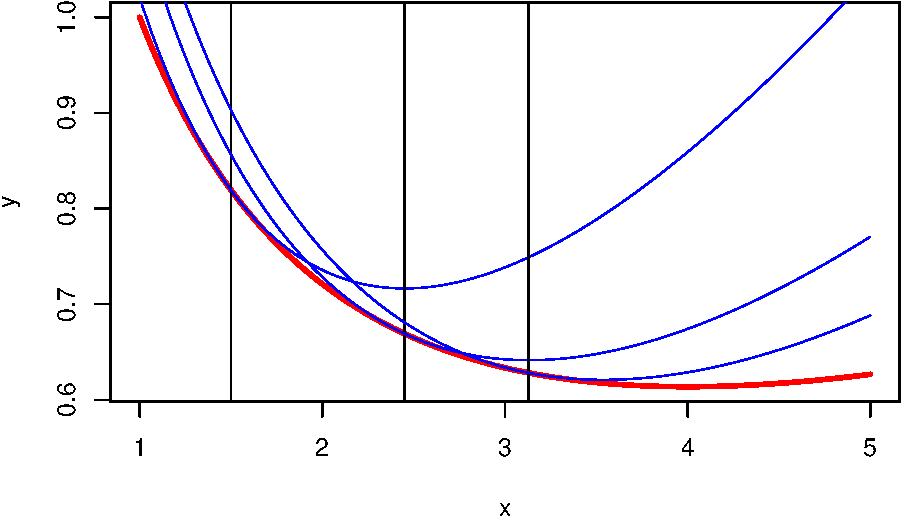
\includegraphics{smacofManual_files/figure-latex/majplot-1} \end{center}

\subsubsection{Majorizing Stress}\label{majorizing-stress}

\subsection{Second Phase: Update Transformation}\label{second-phase-update-transformation}

\subsubsection{Spline Basis Details}\label{spline-basis-details}

\emph{Splines} of degree \(d\) on a closed interval \([a,b]\) are piecewise polynomials of degree \(d\). The endpoints of the interval are the \emph{boundary knots}. In the interval there are a number of \emph{inner knots}. For smacof we suppose the inner knots are distinct. There is a polynomial piece between all consecutive
pairs of knots. Although the pieces can be parts of different polynomials
splines are required to have a certain degree of smoothness. In fact
at the interior knots a spline has \(d - 1\) continuous derivatives. A
spline of degree zero is a step function, stepping to a different level
at each knot. A spline of degree one is piecewise linear, where the
line segments are joined continuously at the inner knots. A spline of
degree two is piecewise quadratic and continuously differentiable at the
knots. And so on. There is no limit on the number of inner knots and
on the degree of the spline, although the number of interior knots
must be greater than or equal to the degree minus one. The flexibility
of the spline (as opposed to the rigidity of a polynomial on \([a,b]\)
of the same degree) comes from the number and placement of the interior knots, not so much from the degree of the spline.

\subsubsection{B-splines}\label{b-splines}

\subsubsection{Berstein PolynomiaLS}\label{berstein-polynomials}

\begin{longtable}[]{@{}ccccc@{}}
\caption{\label{tab:bsplinekable}B spline parameters}\tabularnewline
\toprule\noalign{}
degree & order & ninner & nknots & span \\
\midrule\noalign{}
\endfirsthead
\toprule\noalign{}
degree & order & ninner & nknots & span \\
\midrule\noalign{}
\endhead
\bottomrule\noalign{}
\endlastfoot
0 & 1 & 4 & 6 & 5 \\
1 & 2 & 4 & 8 & 6 \\
2 & 3 & 4 & 10 & 7 \\
3 & 4 & 4 & 12 & 8 \\
4 & 5 & 4 & 14 & 9 \\
\end{longtable}

\[
\sum_i B_{i,k}(x)=1
\]

M-splines

\[
M_{i,k}(x)=\frac{k+1}{t_{i+k+1}-t_i}B_{i,k}(X)
\] then \[
\int M_{i,k}(x)dx=1
\]

I-splines \[
I_{i,k+1}(z)=\int_{-\infty}^zM_{i,k}(x)dx
\]

When is a B-spline increasing ? \[
\mathcal{D}B_{i,k}(x)=
\] Thus if \[
\mathcal{D}\sum_{i=1}^{d+m}\alpha_iB_{i,k}(x)=
\]

It is sufficient that \(\alpha_i\leq\alpha_{i+1}\)

Integral, I-splines

\subsubsection{Ordinal MDS}\label{ordinal-mds}

\subsubsection{Interval and Ratio MDS}\label{interval-and-ratio-mds}

Additive constant

\subsubsection{Cyclic Coordinate Decent}\label{cyclic-coordinate-decent}

In the non-linear least squares (NNLS) problem the data are an
\(n\times p\) matrix \(X\), a vector \(y\) with \(n\) elements, and a positive
semi-definite diagonal matrix \(W\). We want to minimize \[
\sigma(\beta):=\frac12(X\beta-y)'W(X\beta-y)
\] over \(\beta\geq 0\). In data analysis and statistics the problem is
often solved by \emph{active set methods}, implemented in R for example by
NNLS (Mullen and van Stokkum (2023)) and FNNLS (Bro and De Jong (1997)). Active set
methods are finitely convergent dual methods. While iterating the
intermediate solutions are not feasible (i.e.~non-negative). In fact in
dual methods we reach feasibility and optimality at the same time. Also
the number of iterations, although theoretically finite, can be very
large.

In each smacof iteration we need an NNLS solution. Especially in the
early iterations the solution does not have to be very precise. Also the
solution from the previous NNLS problem will generally provide a very
good starting value for the next iteration (each NNLS problem has a ``hot
start''). And finally, we would like all internediate solutions to be
feasible. These considerations have lead us to using \emph{cyclic coordinate
descent} (CCD).

Suppose the current best feasible solution in CCD iteration \(k\) is
\(\beta^{(k)}\). The next CCD iteration changes each of the \(p\)
coordinates of \(\beta^{(k)}\) in turn, maintaining feasibility, while
keeping the other \(p-1\) coordinates fixed at their current values. Thus
within a CCD iteration \(k\) we create intermediate solutions
\(\beta^{(k,1)},\cdots,\beta^{(k,p)}\), where each of the intermediate
solutions \(\beta^{(k,r)}\) differs from the previous one
\(\beta^{(k,r-1)}\) in a single coordinate. For consistency we define
\(\beta^{(k,0)}:=\beta^{(k)}\). After the iteration is finished we set
\(\beta^{(k+1)}=\beta^{(k,p)}\).

Note that in smacof each iteration modifies the coordinates in the order
\(1,\cdots,p\), which explains why the method is called ``cyclic''. There
are variations of CCD in which the order within an iteration is random
or greedy (choose the coordinate which gives the largest improvement) or
zig-zag \(1,\cdots,p,p-1,\cdots,1\). We have not tried out these
alternatives in smacf, but we may in the future.

The effect of changing a single coordinate on the loss function is \[
\sigma(\beta+\epsilon e_j)=\sigma(\beta)+\epsilon\ g_j(\beta)+\frac12\epsilon^2s_{jj},
\] where \(e_j\) is the unit vector corresponding with the coordinate we
are changing, \(g(\beta):=\mathcal{D}\sigma(\beta)=X'Wr(\beta)\) is the
gradient at \(\beta\), and \(r(\beta):=X\beta-y\) is the residual. Also
\(S:=X'WX\). Note that if \(s_{jj}=0\) then also \(g_j(\beta)=0\) and thus
\(\sigma(\beta+\epsilon e_j)=\sigma(\beta)\). In each CCD cycle we simply
skip updating coordinate \(j\).

If \(s_{jj}>0\) then \(\sigma(\beta+\epsilon e_j)\) is a strictly convex
quadratic in \(\epsilon\), which we must minimize under the constraint
\(\beta_j+\epsilon\geq 0\) or \(\epsilon\geq-\beta_j\). Define
\(\hat\epsilon\) to be the solution of this constrained minimization
problem.

The quadratic \ldots{} has its minimum at \[
\tilde\epsilon=-\frac{g_j(\beta)}{s_{jj}}
\] If \(\beta+\tilde\epsilon\) is feasible then it is the update we are
looking for. Thus \(\hat\epsilon=\tilde\epsilon\). If
\(\beta+\tilde\epsilon<0\) then the contrained minimum is attained at the
boundary, i.e.~\(\hat\epsilon=-\beta_j\) and the updated \(\beta_j\) is
zero. Thus, in summary, \(\hat\epsilon=\max(\tilde\epsilon,-\beta_j)\).

One of the nice things about CCD is that \[
r(\hat\beta)=r(\beta)+\hat\epsilon x_j
\] \[
g(\hat\beta)=g(\beta)+\hat\epsilon s_j
\]

It follows that \(\hat\epsilon=0\) if and only if either \(\beta_j=0\) and
\(g_j(\beta)\geq 0\) or if \(g_j(beta)=0\) and \(beta_j>0\).

If \(g_j(\beta)<0\) then \(\tilde\epsilon>0\), and thus \(\hat\epsilon>0\) and
\(\sigma(\hat\beta)<\sigma(\beta)\). Thus we must have \(g_j(\beta)\geq 0\).

If \(\beta_j>0\) and \(g_j(\beta)\not=0\) then there is an \(\epsilon\) such
that \(\sigma(\beta+\epsilon e_j)<\sigma(\beta)\). Thus if \(\beta_j>0\) we
must have \(g_j(\beta)=0\).

In summary at the minimum of \(\sigma\) over \(\beta\geq 0\) we must have
\(\beta_j\geq 0\), \(g_j(\beta)\geq 0\), and \(\beta_jg_j(\beta)=0\) for all
\(j\) (\emph{complementary slackness}).

\[
\sigma(\beta+\epsilon e_j)=\sigma(\beta)+\epsilon\ g_j(\beta)+\frac12\epsilon^2s_{jj},
\] where \(S:=X'WX\).

Now suppose we minimize \(\sigma\) over \(\beta\geq 0\).

Our best solution so far is \(\beta^{(k)}\geq 0\). Minimize
\(\sigma(\beta^{(k)}+\epsilon e_1)\) over \(\epsilon\) on the condition that
\(\beta^{(k)}_1+\epsilon\geq 0\) or \(\epsilon\leq-\beta^{(k)}_1\). If
\(s_{11}=0\) then also \(g_1(\beta)=0\) and we set
\(\beta^{(k+1,1)}=\beta^{(k,1)}\). If \(s_{11}>0\) we compute \[
\tilde\epsilon=-g_1(\beta)/s_{11}
\] If \[
\beta^{(k)}_1+\tilde\epsilon\geq 0
\] then \[
\beta^{(k+1,1)}=\beta^{(k)}_1+\tilde\epsilon
\] If \[
\beta^{(k)}_1+\tilde\epsilon<0
\] we set \[
\beta^{(k+1,1)}=0.
\]

\section{Smacof Program}\label{smacof-program}

\subsubsection{Front-end}\label{front-end}

The front-end for both smacofRR and smacofRC is written in R. The
analysis is started in the user's working directory by the command
smacofRR(foo) or smacofRC(foo), where foo is a user-chosen name (without
quotes).

Two text files need to be present in the working directory. The first is
fooParameters.txt, where of course you substitute the user-chosen name
for foo. The second file is fooDelta.txt, which has the dissimilarities
below the diagonal in row-major order.

The parameter file has key-value format. Here is an example.

\begin{Shaded}
\begin{Highlighting}[]
\NormalTok{nobj   }\DecValTok{9}
\NormalTok{ndim   }\DecValTok{3}
\NormalTok{init   }\DecValTok{2}
\NormalTok{width   }\DecValTok{10}
\NormalTok{precision   }\DecValTok{6}
\NormalTok{haveweights   }\DecValTok{0}
\NormalTok{itmax  }\DecValTok{1000}
\NormalTok{epsi  }\DecValTok{10}
\NormalTok{verbose  }\DecValTok{1}
\NormalTok{ditmax  }\DecValTok{5}
\NormalTok{depsi  }\DecValTok{6}
\NormalTok{dverbose  }\DecValTok{0}
\NormalTok{kitmax  }\DecValTok{5}
\NormalTok{kepsi  }\DecValTok{6}
\NormalTok{kverbose  }\DecValTok{0}
\NormalTok{degree  }\DecValTok{3}
\NormalTok{haveknots  }\DecValTok{3}
\NormalTok{ninner  }\DecValTok{5}
\NormalTok{ordinal  }\DecValTok{1}
\NormalTok{anchor }\DecValTok{0}
\NormalTok{intercept  }\DecValTok{1}
\end{Highlighting}
\end{Shaded}

The parameter file is read first, using the R function read.table().
There is one key-value pair on each line, at the start of the line. The order of the lines does not matter. There can be additional comments or other text on
each line after the value field, as long as that text is space-separated
from the value field. Additional key-value lines with non-existing
parameters can be added at will.

Values of the parameters are put the local environment using R function
assign(), which means they are available to R throughout the smacof run.
Of course if we choose smacofRC the front-end needs to pass them to C
using C(), but they will be available again for the back-end.

The Delta file, and any subsequent optional input files, are read with
the R function scan(). Values are separated by spaces. They can be on a
single line, or laid out as a lower-triangular matrix, or whatever. The
function scan() only stops reading if it reaches the end-of-file.

We'll now discuss the parameters one by one. Note that all parameters
are integers. The first two are obvious: \emph{nobj} is the number of objects
and \emph{ndim} the number of dimensions. These two parameters have no
default or recommended values, because they deyermined by the data. All
other parameters in our example parameter file are set to reasonable
values in our example parameter file. But the whole idea is to
experiment with various combinations of parameter values, so
``reasonable'' is weaker than ``recommended'' and ``recommended'' is weaker
than ``default''.

The \emph{init} parameter can have values 1, 2, or 3. If \emph{init} equals 1 the
program reads an initial configuration from the file fooXinit.txt in the
working directory. The file has \emph{nobj} * \emph{ndim} numbers, the initial
configuration, in row-major format. If \emph{init} = 2 then the classical
Torgerson initial estimate will be computed. If \emph{init} = 3 a random
initial estimate will be used.

\emph{width} and \emph{precision} are parameters for the output of the values of
stress during iterations.

\emph{haveweights} is either zero or one. If zero there are no weights, which
is equivalent to all weights equal to one. If one then we will read a
file fooWeights.txt, which has the lower-diagonal \(\frac12 n(n-1)\)
weights in row-major order.

As explained in previous sections there are three iterative running in
smacof. There are two inner iterations: one for the configuration for
fixed disparities, and one for the disparities for fixed configuration.
The two inner iteration loops are nested in one outer iteration loop.
Each of the iterations has three parameters: one for the maximum number
of iterations, one for the stopping criterion, and one for the verbosity
of the iteration output. For the outer loop the parameters are \emph{itmax},
\emph{ieps}, and \emph{verbose}. For the inner configuration loop they are
\emph{kitmax}, \emph{keps}, and \emph{kverbose}. And the inner transformation loop they
are \emph{ditmax}, \emph{deps}, and \emph{dverbose}. If the verbose parameter is one,
then each iteration prints out the stress before and the stress after
update. If verbose is zero, nothing is printed. The stopping parameters
check if the change in stress in an iteration is less than epsilon,
where epsilon is 10\^{}-ieps, 10\^{}-keps, or 10\^{}-deps.

The final five parameters are used to define the nature of the spline
space for the transformations. \emph{degree} is the degree of the piecewise
polynomials. The \emph{haveknots} parameter can be 0, 1, 2, or 3. If it is
zero, there are no inner knots and we use the Bernstein polynomial
basis. If \emph{haveknots} is one, the inner knots are read in from
fooKnots.txt in the usual way. If \emph{haveknots} is two the knots are
equally spaced between zero and one, and if it is three the knots are
equally spaced on the precentile scale (so that the number of data
points between knots is approximately the same). The \emph{ninner} parameter
determines the number of knots in the case that \emph{haveknots} is either
two or three. If \emph{haveknots} is zero, then \emph{ninner} should be zero, if
\emph{haveknots} is one it should be equal to the number of knots in
fooKnots.txt.

The three final spline parameters are \emph{ordinal}, \emph{anchor}, and \emph{intercept}. If \emph{ordinal} is one the fitted spline is constrained to be monotone. If \emph{intercept} is zero then the first spline coefficient is constrained to be zero (which
means the first column is deleted from the basis). This means that the spline
is constrained to be zero at the lower boundary knot. If \emph{intercept} is one
there is no such constraint, and the spline can be anything at the lower boundary
(subject to monotonicity of \emph{ordinal} is one). If \emph{anchor} is one then the
boundary knots are set to zero and the maximum dissimilarity, if \emph{anchor} is
zero the boundary knots are the minimum and maximum dissimilarity. Thus if \emph{intercept} is zero and \emph{anchor} is one the spline goes through the origin.

The computations in the frontend are straightforward. We first transform
the dissimilarities linearly so that the smallest becomes zero and the
largest becomes one. This is not strictly necessary but it makes the
spline computations slightly easier.

Initial Estimates for \(X\) Spline Basis

\subsubsection{Engine}\label{engine}

ALS First Phase Second Phase

\subsubsection{Back-end}\label{back-end}

The back-end consists of a number of R functions that have the list
returned by smacofRR or smacofRC as an argument. They can be used to
make plots, compute derivatives, convert matrices to an easily
printable format, do sensitivity analysis, and so on. The philosophy
is that in the backend the main computing is finished and we
just create different representations of the results.

\paragraph{Plotting}\label{plotting}

There are two main plot functions in the backend: smacofShepardPlot()
and smacofConfigurationPlot(). A smacofShepardPlot has the
dissimilarities (un-normalized) on the horizontal axes and
it has the distances and the disparities on the vertical axis.
It draws the spline, and shows where the fitted disparities are
on the spline. It also plots the (delta, dist) pairs as points,
to show how far they deviate from the spline. Optionally
smacofShepardPlot() can draw vertical lines at the inner knots
(argument knotlines = TRUE), and optionally it can connect
the (delta, dhat) points on the spline to the (delta, dist)
points with lines (argument fitlines = TRUE).

It must be emphasized that smacofShepardPlot() draws the spline
over the whole interval, which is either (deltamin, deltamax)
if anchor = 0 and (0, deltamax) if anchor = 1. It does
this by recomputing the spline at a large number of
uniformly spaced points in the interval, where the
number of points is given by the smacofShepardPlot()
parameter resolution. Thus we do not use only the
data points (delta,dhat) and then let the R plot function
interpolate linearly. That can be misleading. It is
especially misleading if degree is zero (step function)
or if there are consecutive inner knots with no data values
between the knots. Degree zero is handled by the special
purpose step function plotting routine smacofPlotStepFunction(),
which makes sure the spline is drawn as a horizontal segment
from one knot to the next knot. In addition smacofShepardPlot()
can set some base R plot parameters such as col, cex, lwd, and pch
(see the R documentation).

The smacofConfigurationPlot() function is much simpler than
smacofShepardPlot(). It sets pch, col, and cex. It uses
the smacofRR/RC labels parameter to decide how to label
the points in the configuration. If labels = 1 it reads
a character vector of labels from fooLabels.txt, where
foo is of course the name of the run. If labels = 2
the points are numbered, if labels = 3 plotting uses
the pch symbol for all points. If the dimension \(p\)
is larger than two, smacofConfigurationPlot() uses
the parameters dim1 and dim2 to select the dimensions
to plot.

\paragraph{Writing}\label{writing}

\paragraph{Checking}\label{checking}

\paragraph{Derivatives}\label{derivatives-1}

\paragraph{Sensitivity}\label{sensitivity}

Perturbation regions

Parametric Bootstrap

Jacknife

\section{Examples}\label{examples}

\subsection{ekman}\label{ekman}

The Ekman (1954) color circle example has been used in many, if not most, multidimensional scaling textbooks and review articles. This is due, no doubt,
to its astonishing good two-dimensional fit and its easy interpretability.

\begin{greybox}

\begin{center}
\textbf{INSERT TABLE \ref{tab:ekmankable} ABOUT HERE}

\end{center}

\end{greybox}

\begin{greybox}

\begin{center}
\textbf{INSERT FIGURE \ref{fig:ekmancubic} ABOUT HERE}

\end{center}

\end{greybox}

\begin{greybox}

\begin{center}
\textbf{INSERT FIGURE \ref{fig:ekmanordinal} ABOUT HERE}

\end{center}

\end{greybox}

\subsection{gruijter}\label{gruijter}

The two previous examples had a good fit. We use the data from De Gruijter (1967)
for an example with a rather bad fit in two dimensions and a rather good fit in three dimensions.
Dissimilarity judgments between nine Dutch political parties were
collected in 1966 by the complete method of triads. Results were
averaged over 100 students. Averaging over a heterogeneous population
will cause regression to the mean, and thus dissimilarities will tend
to be more equal than they should be on the basis of the individual
results. This means there should be a large difference in fit between
the ``ratio'' and the ``interval'' options
(i.e.~between the interval parameter equal to one or zero).

\subsection{morse}\label{morse}

\section{Tables}\label{tables}

\begin{longtable}[]{@{}
  >{\centering\arraybackslash}p{(\columnwidth - 16\tabcolsep) * \real{0.0988}}
  >{\centering\arraybackslash}p{(\columnwidth - 16\tabcolsep) * \real{0.0988}}
  >{\centering\arraybackslash}p{(\columnwidth - 16\tabcolsep) * \real{0.1358}}
  >{\centering\arraybackslash}p{(\columnwidth - 16\tabcolsep) * \real{0.1111}}
  >{\centering\arraybackslash}p{(\columnwidth - 16\tabcolsep) * \real{0.1358}}
  >{\centering\arraybackslash}p{(\columnwidth - 16\tabcolsep) * \real{0.0988}}
  >{\centering\arraybackslash}p{(\columnwidth - 16\tabcolsep) * \real{0.0741}}
  >{\centering\arraybackslash}p{(\columnwidth - 16\tabcolsep) * \real{0.1728}}
  >{\centering\arraybackslash}p{(\columnwidth - 16\tabcolsep) * \real{0.0741}}@{}}
\caption{\label{tab:ekmankable}Analyses of the ekman example}\tabularnewline
\toprule\noalign{}
\begin{minipage}[b]{\linewidth}\centering
ninner
\end{minipage} & \begin{minipage}[b]{\linewidth}\centering
degree
\end{minipage} & \begin{minipage}[b]{\linewidth}\centering
haveknots
\end{minipage} & \begin{minipage}[b]{\linewidth}\centering
ordinal
\end{minipage} & \begin{minipage}[b]{\linewidth}\centering
intercept
\end{minipage} & \begin{minipage}[b]{\linewidth}\centering
anchor
\end{minipage} & \begin{minipage}[b]{\linewidth}\centering
ndim
\end{minipage} & \begin{minipage}[b]{\linewidth}\centering
stress
\end{minipage} & \begin{minipage}[b]{\linewidth}\centering
itel
\end{minipage} \\
\midrule\noalign{}
\endfirsthead
\toprule\noalign{}
\begin{minipage}[b]{\linewidth}\centering
ninner
\end{minipage} & \begin{minipage}[b]{\linewidth}\centering
degree
\end{minipage} & \begin{minipage}[b]{\linewidth}\centering
haveknots
\end{minipage} & \begin{minipage}[b]{\linewidth}\centering
ordinal
\end{minipage} & \begin{minipage}[b]{\linewidth}\centering
intercept
\end{minipage} & \begin{minipage}[b]{\linewidth}\centering
anchor
\end{minipage} & \begin{minipage}[b]{\linewidth}\centering
ndim
\end{minipage} & \begin{minipage}[b]{\linewidth}\centering
stress
\end{minipage} & \begin{minipage}[b]{\linewidth}\centering
itel
\end{minipage} \\
\midrule\noalign{}
\endhead
\bottomrule\noalign{}
\endlastfoot
0 & 3 & 0 & 1 & 0 & 1 & 2 & 0.0021309760 & 39 \\
5 & 3 & 3 & 1 & 0 & 1 & 2 & 0.0008780736 & 1260 \\
50 & 0 & 3 & 1 & 0 & 1 & 2 & 0.0005138551 & 877 \\
50 & 0 & 2 & 1 & 0 & 1 & 2 & 0.0010662271 & 492 \\
\end{longtable}

\begin{center}\rule{0.5\linewidth}{0.5pt}\end{center}

\begin{center}\rule{0.5\linewidth}{0.5pt}\end{center}

\section{Figures}\label{figures}

\begin{figure}

{\centering 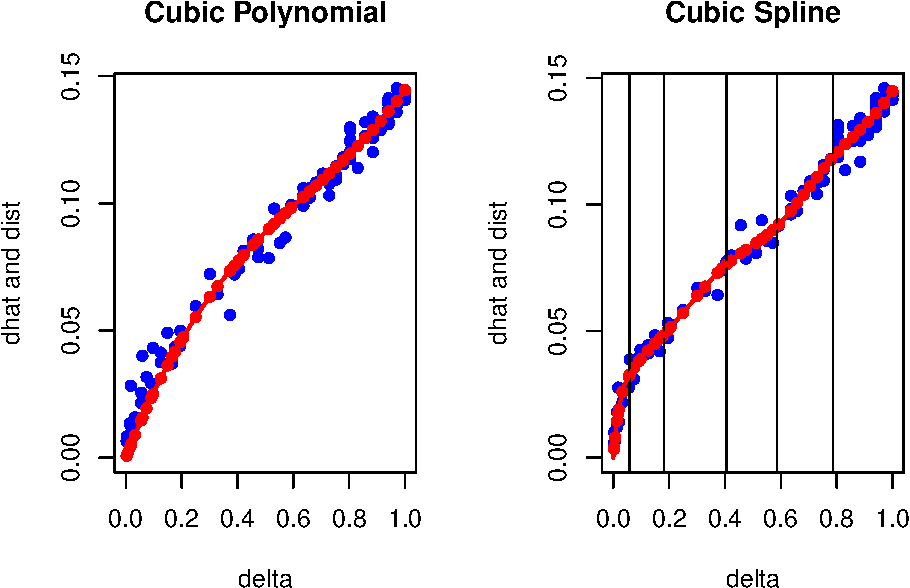
\includegraphics{smacofManual_files/figure-latex/ekmancubic-1} 

}

\caption{Ekman example, cubic analysis}\label{fig:ekmancubic}
\end{figure}

\begin{figure}

{\centering 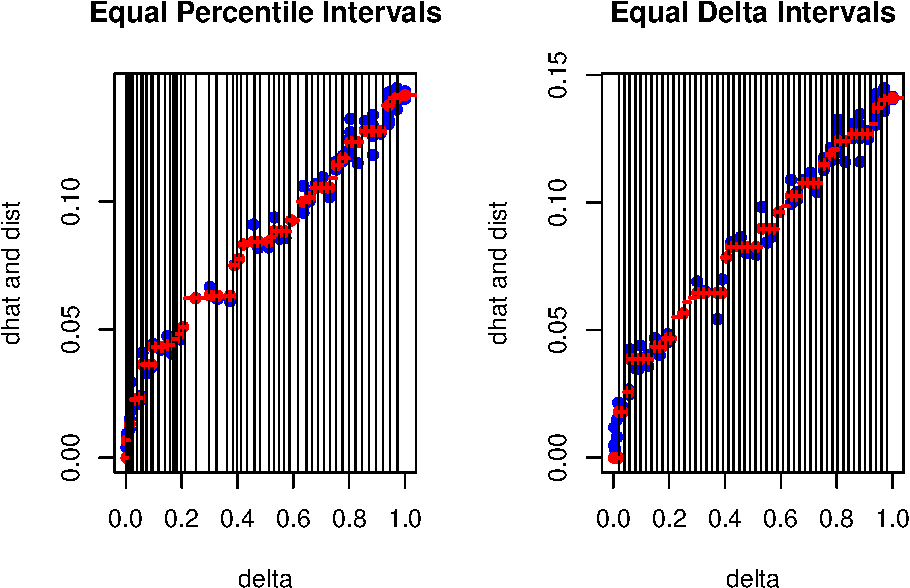
\includegraphics{smacofManual_files/figure-latex/ekmanordinal-1} 

}

\caption{Ekman example, nonmetric analysis}\label{fig:ekmanordinal}
\end{figure}

\section*{References}\label{references}
\addcontentsline{toc}{section}{References}

\phantomsection\label{refs}
\begin{CSLReferences}{1}{0}
\bibitem[\citeproctext]{ref-bauschke_bui_wang_18}
Bauschke, H. H., M. N. Bui, and X. Wang. 2018. {``{Projecting onto the Intersection of a Cone and a Sphere}.''} \emph{SIAM Journal on Optimization} 28: 2158--88.

\bibitem[\citeproctext]{ref-boehning_lindsay_88}
Böhning, D., and B. G. Lindsay. 1988. {``{Monotonicity of Quadratic-approximation Algorithms}.''} \emph{Annals of the Institute of Statistical Mathematics} 40 (4): 641--63.

\bibitem[\citeproctext]{ref-bro_dejong_97}
Bro, R., and S. De Jong. 1997. {``A Fast Non-Negatively-Constrained Least Squares Algorithm.''} \emph{Journal of Chemometrics} 11: 393--401.

\bibitem[\citeproctext]{ref-degruijter_67}
De Gruijter, D. N. M. 1967. {``{The Cognitive Structure of Dutch Political Parties in 1966}.''} Report E019-67. Psychological Institute, University of Leiden.

\bibitem[\citeproctext]{ref-deleeuw_U_75a}
De Leeuw, J. 1975. {``{A Normalized Cone Regression Approach to Alternating Least Squares Algorithms}.''} Department of Data Theory FSW/RUL.

\bibitem[\citeproctext]{ref-deleeuw_C_77}
---------. 1977. {``Applications of Convex Analysis to Multidimensional Scaling.''} In \emph{Recent Developments in Statistics}, edited by J. R. Barra, F. Brodeau, G. Romier, and B. Van Cutsem, 133--45. Amsterdam, The Netherlands: North Holland Publishing Company.

\bibitem[\citeproctext]{ref-deleeuw_A_84f}
---------. 1984. {``{Differentiability of Kruskal's Stress at a Local Minimum}.''} \emph{Psychometrika} 49: 111--13.

\bibitem[\citeproctext]{ref-deleeuw_C_94c}
---------. 1994. {``{Block Relaxation Algorithms in Statistics}.''} In \emph{Information Systems and Data Analysis}, edited by H. H. Bock, W. Lenski, and M. M. Richter, 308--24. Berlin: Springer Verlag. \url{https://jansweb.netlify.app/publication/deleeuw-c-94-c/deleeuw-c-94-c.pdf}.

\bibitem[\citeproctext]{ref-deleeuw_U_14b}
---------. 2014. {``{Bounding, and Sometimes Finding, the Global Minimum in Multidimensional Scaling}.''} UCLA Department of Statistics. \url{https://jansweb.netlify.app/publication/deleeuw-u-14-b/deleeuw-u-14-b.pdf}.

\bibitem[\citeproctext]{ref-deleeuw_E_17q}
---------. 2017a. {``{Pseudo Confidence Regions for MDS}.''} 2017. \url{https://jansweb.netlify.app/publication/deleeuw-e-17-q/deleeuw-e-17-q.pdf}.

\bibitem[\citeproctext]{ref-deleeuw_E_17e}
---------. 2017b. {``{Shepard Non-metric Multidimensional Scaling}.''} 2017. \url{https://jansweb.netlify.app/publication/deleeuw-e-17-e/deleeuw-e-17-e.pdf}.

\bibitem[\citeproctext]{ref-deleeuw_E_19d}
---------. 2019. {``Normalized Cone Regression.''} 2019. \url{https://jansweb.netlify.app/publication/deleeuw-e-19-d/deleeuw-e-19-d.pdf}.

\bibitem[\citeproctext]{ref-deleeuw_mair_A_09c}
De Leeuw, J., and P. Mair. 2009. {``{Multidimensional Scaling Using Majorization: SMACOF in R}.''} \emph{Journal of Statistical Software} 31 (3): 1--30. \url{https://www.jstatsoft.org/article/view/v031i03}.

\bibitem[\citeproctext]{ref-dempster_laird_rubin_77}
Dempster, A. P., N. M. Laird, and D. B. Rubin. 1977. {``{Maximum Likelihood for Incomplete Data via the EM Algorithm}.''} \emph{Journal of the Royal Statistical Society} B39: 1--38.

\bibitem[\citeproctext]{ref-ekman_54}
Ekman, G. 1954. {``{Dimensions of Color Vision}.''} \emph{Journal of Psychology} 38: 467--74.

\bibitem[\citeproctext]{ref-fang_oleary_12}
Fang, H., and D. P. O'Leary. 2012. {``Euclidean Distance Matrix Completion Problems Euclidean Distance Matrix Completion Problems Euclidean Distance Matrix Completion Problems.''} \emph{Oprtimization Methods and Software} 27 (4-5): 695--717.

\bibitem[\citeproctext]{ref-guttman_68}
Guttman, L. 1968. {``{A General Nonmetric Technique for Fitting the Smallest Coordinate Space for a Configuration of Points}.''} \emph{Psychometrika} 33: 469--506.

\bibitem[\citeproctext]{ref-kruskal_64a}
Kruskal, J. B. 1964a. {``{Multidimensional Scaling by Optimizing Goodness of Fit to a Nonmetric Hypothesis}.''} \emph{Psychometrika} 29: 1--27.

\bibitem[\citeproctext]{ref-kruskal_64b}
---------. 1964b. {``{Nonmetric Multidimensional Scaling: a Numerical Method}.''} \emph{Psychometrika} 29: 115--29.

\bibitem[\citeproctext]{ref-kruskal_carroll_69}
Kruskal, J. B., and J. D. Carroll. 1969. {``{Geometrical Models and Badness of Fit Functions}.''} In \emph{Multivariate Analysis, Volume II}, edited by P. R. Krishnaiah, 639--71. North Holland Publishing Company.

\bibitem[\citeproctext]{ref-lange_16}
Lange, K. 2016. \emph{MM Optimization Algorithms}. SIAM.

\bibitem[\citeproctext]{ref-lethi_tao_18}
Le Thi, H. A., and P. D. Tao. 2018. {``{DC Programming and DCA: Thirty Years of Developments}.''} \emph{Mathematical Programming, Series B}.

\bibitem[\citeproctext]{ref-mair_groenen_deleeuw_A_22}
Mair, P., P. J. F. Groenen, and J. De Leeuw. 2022. {``{More on Multidimensional Scaling in R: smacof Version 2}.''} \emph{Journal of Statistical Software} 102 (10): 1--47. \url{https://www.jstatsoft.org/article/view/v102i10}.

\bibitem[\citeproctext]{ref-mullen_vanstokkum_23}
Mullen, K. M., and I. H. M. van Stokkum. 2023. \emph{{nnls: The Lawson-Hanson algorithm for non-negative least squares (NNLS)}}. \url{\%7Bhttps://CRAN.R-project.org/package=nnls\%7D}.

\bibitem[\citeproctext]{ref-nikolova_ng_05}
Niikolova, M., and M. Ng. 2005. {``Analysis of Half-Quadratic Minimization Methods for Signal and Image Recovery.''} \emph{SIAM Journal Scientific Computing} 27 (3): 937--66.

\bibitem[\citeproctext]{ref-shepard_62a}
Shepard, R. N. 1962a. {``{The Analysis of Proximities: Multidimensional Scaling with an Unknown Distance Function. I}.''} \emph{Psychometrika} 27: 125--40.

\bibitem[\citeproctext]{ref-shepard_62b}
---------. 1962b. {``{The Analysis of Proximities: Multidimensional Scaling with an Unknown Distance Function. II}.''} \emph{Psychometrika} 27: 219--46.

\bibitem[\citeproctext]{ref-vosz_eckhardt_80}
Vosz, H., and U. Eckhardt. 1980. {``{Linear Convergence of Generalized {W}eiszfeld's Method}.''} \emph{Computing} 25: 243--51.

\bibitem[\citeproctext]{ref-yuille_rangarajan_03}
Yuille, A. L., and A. Rangarajan. 2003. {``{The Concave-Convex Procedure}.''} \emph{Neural Computation} 15: 915--36.

\bibitem[\citeproctext]{ref-zangwill_69a}
Zangwill, W. I. 1969. \emph{{Nonlinear Programming: a Unified Approach}}. Englewood-Cliffs, N.J.: Prentice-Hall.

\end{CSLReferences}

\end{document}
